\PassOptionsToPackage{colorlinks=true,linkcolor=blue,citecolor=blue,urlcolor=blue}{hyperref}
% REQ-FILE: The above line, \PassOptionsToPackage{} must be very first line.

\documentclass[11pt]{article}

% Encoding and font setup for cross-platform reproducibility
\usepackage[utf8]{inputenc}
\usepackage[T1]{fontenc}
\usepackage{lmodern}

% Improve readability for dense theoretical material
\usepackage{setspace}
\onehalfspacing

% Mathematical notation and table formatting for formal semantics
\usepackage{amsmath, amssymb}
\usepackage{booktabs}
\usepackage{bookmark}
\usepackage{graphicx}

% Theorem environments for definitions, lemmas, and formal statements
\usepackage{amsthm}

% plain style is italic body text (for theorems, lemmas, etc.)
\theoremstyle{plain}
\newtheorem{theorem}{Theorem}[section]
\newtheorem{lemma}[theorem]{Lemma}
\newtheorem{proposition}[theorem]{Proposition}
\newtheorem{corollary}[theorem]{Corollary}
\newtheorem{conjecture}[theorem]{Conjecture}

% definition style = upright body text (for definitions, examples)
\theoremstyle{definition}
\newtheorem{definition}[theorem]{Definition}
\newtheorem{example}[theorem]{Example}

% remark style = upright, lighter weight (for remarks, notes)
\theoremstyle{remark}
\newtheorem{remark}[theorem]{Remark}
\newtheorem{note}[theorem]{Note}

% Bibliography management and hyperlink support
\usepackage{url}
\usepackage{hyperref}
\usepackage{natbib}

% Support multiple author affiliations
\usepackage{authblk}

% Improve typographic quality and line breaking
\usepackage{microtype}

% Categorical and commutative diagrams
\usepackage{tikz}
\usepackage{tikz-cd}
\usetikzlibrary{arrows.meta,calc,fit,positioning,shapes.geometric}

% Callout boxes for examples and emphasis
\usepackage{mdframed}
\usepackage[most]{tcolorbox}

% Keywords macro for structured abstract metadata
\providecommand{\keywords}[1]{\textbf{Keywords: } #1}

% Notation for Raw vs Canonical categories in CEP/CEE
\newcommand{\Raw}{\mathsf{Raw}}
\newcommand{\Canon}{\mathsf{Canon}}

% Reusable figure callout box for visual emphasis
\newcommand{\FigureCallout}[2]{%
  \begin{tcolorbox}[
    colback=gray!5,
    colframe=black!40,
    title={#1},
    fonttitle=\bfseries,
    arc=3pt,
    boxrule=0.5pt,
    width=\linewidth,
    enhanced,
    breakable
  ]
  #2
  \end{tcolorbox}
}

% Paragraph spacing prioritizes readability over traditional indentation
\setlength{\parskip}{0.75em}
\setlength{\parindent}{0em}

% Compact list formatting for dense conceptual content
\usepackage{enumitem}
\setlist[itemize]{itemsep=0.2em, topsep=0.2em, parsep=0em, partopsep=0em}

% Defensive re-definition ensures commands exist if loaded earlier
\providecommand{\Raw}{\mathrm{Raw}}
\providecommand{\Canon}{\mathrm{Canon}}

\title{A Categorical Semantics for the Civic Exchange Protocol (CEP)}

\author[1,2]{Denise M. Case}
\affil{Northwest Missouri State University, Computer Science and Information Systems, Maryville, MO, USA \\
       Civic Interconnect, Ely, MN, USA}

\date{\today}

\begin{document}

\maketitle
\vspace{-1em}

% Explicitly mark preprint status
\begin{tcolorbox}[colback=gray!10, colframe=black!20, boxrule=0.3pt]
    \textbf{Preprint Notice.}
    This preprint has not undergone peer review.
    It is shared to support community discussion, transparency research, and early technical evaluation.
\end{tcolorbox}

\begin{abstract}
    The Civic Exchange Protocol (CEP) defines entities, relationships, exchanges,
    and context tags as foundational primitives for civic information systems~\cite{case2025cep}.
    This paper develops a categorical semantics for CEP, providing a rigorous
    mathematical basis for its compositional structure, identity guarantees,
    and interoperability claims.
    CEP records are modeled as typed objects in a finitely complete category,
    with morphisms representing provenance-preserving transformations.
    Envelopes, attestations, and context tags arise as natural transformations
    between functors encoding system-level views of the data.
    Canonicalization is formulated as a strict monoidal functor that preserves
    identity and equivalence classes, while jurisdictional adapters appear as
    oplax functors mediating between local schemas and global vocabularies.
    Together, these constructions clarify CEP's invariants, formalize correctness
    properties of its identifier mechanism (SNFEI),
    and establish a robust foundation for future work in verification,
    data fusion, and cross-jurisdiction interoperability.
\end{abstract}

\begin{keywords}
    Civic data;
    category theory;
    functorial data modeling;
    interoperability;
    canonicalization;
    identifiers;
    provenance.
\end{keywords}

% !TeX root = 00P1_cae_ontology.tex

\section{Introduction and Motivation}
\label{sec:introduction}

Civic systems are governed by complex interactions among laws, institutions,
infrastructure, financial flows, and measured outcomes.
Data describing these systems is typically fragmented across domains such as procurement, public
health, environmental regulation, education, and infrastructure.
While each domain is often supported by mature data systems, the structural relationships
that connect authority, obligation, action, and long-term outcomes are
rarely represented in a unified or
interoperable form~\cite{bowker2000sorting,edwards2011infrastructure}.

This fragmentation presents a fundamental obstacle to accountability and
longitudinal analysis.
Short-term metrics are frequently privileged over
long-term public value, and outcomes that accrue over decades—such as population
health, infrastructure resilience, or environmental quality—are difficult to
relate back to the legal, institutional, and financial decisions that shape
them~\cite{edwards2011infrastructure,kahn2002information}.
As a result, public investments with high upfront costs and diffuse
benefits are systematically undervalued, even when their historical impact is
well established.

Many existing approaches focus either on transactional data (such as payments
or contracts), legal texts (such as statutes and regulations), or outcome
measures (such as health or economic indicators).
Few provide a principled way to connect these elements without
collapsing distinct concepts into a single
layer or embedding interpretive assumptions directly into data models~\cite{bowker2000sorting}.

This paper introduces the Civic Accountable Entities (CAE) ontology as a
foundational response to this challenge.
CAE defines a formal ontology of entities that participate in
obligations, authority, and accountability within civic systems.
Rather than modeling domains or sectors directly, CAE identifies
a small set of disjoint entity kinds that are stable across time and context and
sufficient to represent the structural relationships underlying civic accountability.

The design of CAE emphasizes ontological clarity over descriptive completeness.
Entities are partitioned into disjoint kinds with explicit identity criteria;
roles, classifications, and sectoral labels are modeled as attributes or
relationships rather than as entity kinds.
This discipline prevents ontological overlap and supports formal reasoning
about obligations, authority, and evidence.

CAE draws on foundational work in formal ontology, particularly the
emphasis on rigorous categorization found in BFO~\cite{smith2015bfo} and
DOLCE~\cite{masolo2004wonderweb}, while making commitments tailored to
civic accountability: entities are included in CAE only insofar as they
participate in accountability-bearing relationships, and the ontology
is designed to remain stable as domains, policies, and tooling evolve.
Section~\ref{sec:related} discusses these relationships in detail.

CAE provides the ontological foundation for the Civic Exchange Protocol (CEP),
which models how entities exchange value and authority, and for Contextual
Evidence and Explanations (CEE), which attaches structured explanations to
civic decisions.
By separating what exists from how it moves and how decisions are explained,
CAE enables interoperable, auditable, and longitudinal analysis of public
systems while remaining neutral with respect to policy positions or causal claims.

The remainder of this paper is organized as follows:
Section~\ref{sec:related} situates CAE within related work in formal ontology;
Section~\ref{sec:principles} outlines the design principles and scope
of CAE;
Section~\ref{sec:ontology} defines the six disjoint entity kinds;
Section~\ref{sec:relationships} discusses relationships and structural constraints;
Section~\ref{sec:evaluation} evaluates CAE via competency questions;
Section~\ref{sec:laws} discusses laws, regulations, and accountability chains;
Section~\ref{sec:outcomes} discusses outcomes, observations, and public value;
Section~\ref{sec:discussion} includes discussion and future work;
and Section~\ref{sec:conclusion} provides a conclusion.
              % Introduction and Motivation
% !TeX root = 00P2_cep_semantics.tex

\section{Preliminaries}
\label{sec:preliminaries}

This section reviews the mathematical tools used throughout the
paper and summarizes the structural elements of the Civic Exchange
Protocol (CEP).
We assume only standard familiarity with category theory,
drawing primarily from Mac~Lane~\cite{maclane1971categories}
and Spivak~\cite{spivak2014category} for the treatment of categories
as models of data and structure-preserving transformations.

% ------------------------------------------------------------
\subsection{Category-Theoretic Background}
% ------------------------------------------------------------

We recall only the categorical notions required for the development of
CEP semantics:

\begin{itemize}
  \item \textbf{Categories}: collections of objects and morphisms equipped with associative composition and identity arrows.

  \item \textbf{Functors}: structure-preserving mappings between categories,
        sending objects to objects and morphisms to morphisms
        in a way that respects identities and composition.

  \item \textbf{Natural transformations}: morphisms between
        functors, providing coherent comparisons between system-level
        views of the same underlying data.

  \item \textbf{Monoidal categories}: categories equipped with a
        tensor product $\otimes$ and unit object $I$, allowing formal
        reasoning about concatenation, aggregation, and combination of
        structured data streams.

  \item \textbf{Oplax functors}: functors that preserve monoidal or
        structural properties up to a controlled relaxation, used here to
        model schema adapters that preserve meaning even when strict
        equivalence between jurisdictions cannot be enforced.
\end{itemize}

These constructions provide a natural language for expressing CEP's
compositional structure:
canonicalization becomes a monoidal functor,
envelopes become natural transformations, and adapters become oplax
mediators between local and global schema categories.

% ------------------------------------------------------------
\subsection{CEP Structural Recap}
% ------------------------------------------------------------

CEP defines four record families:

\begin{itemize}
  \item \textbf{Entities}: civic actors (organizations, agencies, districts, individuals).

  \item \textbf{Relationships}: directed or undirected structural
        links between entities (membership, control, affiliation, reporting lines).

  \item \textbf{Exchanges}: flows of value, information, or action
        between entities (payments, transfers, notifications).

  \item \textbf{Context tags}: optional, non-canonical annotations
        that express interpretive, analytic, or contextual facts about a record.
\end{itemize}

All record families are wrapped in a shared \emph{record envelope}
that provides:

\begin{itemize}
  \item schema and vocabulary references,
  \item revision numbers and lifecycle status,
  \item attestation metadata,
  \item timestamps describing observation and validity intervals,
  \item stable CEP identifiers (verifiable IDs).
\end{itemize}

The envelope separates canonical, identity-bearing components of a
record from contextual or analytic metadata, ensuring both stability
and extensibility.

% ------------------------------------------------------------
\subsection{The A-I-E Criterion}
% ------------------------------------------------------------

Not all civic data qualifies for inclusion in the CEP category.
We formalize the admission criterion as follows:

\begin{definition}[Admissible-Identifiable-Exchangeable (A-I-E)]
  \label{def:aie}
  A civic data record satisfies the \emph{A-I-E criterion} if and only if:
  \begin{enumerate}
    \item \textbf{Admissible (A)}: The record conforms to a declared CEP schema
          and passes validation against its \texttt{recordSchemaUri}.
          The payload instantiates one of the six CAE entity kinds (Actor, Site,
          Instrument, Event, Jurisdiction, Observation) or a valid relationship
          or exchange between such entities.

    \item \textbf{Identifiable (I)}: The record's canonical payload produces a
          stable identifier under CEP canonicalization---either a registry ID
          (LEI, SAM UEI, etc.) or a derived SNFEI when no registry ID is available.

    \item \textbf{Exchangeable (E)}: The record is wrapped in a valid envelope
          with attestation, timestamp, and revision metadata sufficient for
          provenance-preserving exchange across system boundaries.
  \end{enumerate}
\end{definition}

The A-I-E criterion acts as a \emph{filter}: it determines which records
from heterogeneous civic data sources may be lifted into $\mathbf{CEP}$.
Records failing any condition are excluded from the category until
remediated by canonicalization, schema alignment, or envelope construction.

% ------------------------------------------------------------
\subsection{Canonicalization and Identifiers}
% ------------------------------------------------------------


For entity records, CEP constructs a canonical string from
jurisdiction-normalized components such as name, address, and
formation date.
A SHA-256 hash of this canonical string yields a
stable identifier known as the \emph{Structured Non-Fungible Entity Identifier} (SNFEI).

In this paper, we treat canonicalization as a deterministic, strictly monoidal process:
concatenation of components corresponds to a tensor-like operation, and hashing
corresponds to an endofunctor that collapses equivalence classes of canonical strings
to identity objects.
This perspective will be formalized in Section~\ref{sec:canonicalization}.

The stability of SNFEIs under valid record transformations is a core invariant
that underpins CEP's interoperability guarantees.

The formal semantics developed in subsequent sections establish the precise
conditions under which this stability holds.
      % Category Theory Background
% !TeX root = 00P3_cee_verticals.tex

\section{Recap of the CEP Canonical Layer}
\label{sec:cep-recap}

The first paper in this series develops CEP as a rewriting-based,
categorical framework for civic data.
Here we briefly recap the aspects that are most relevant for
vertical domains and civic explanations.

% ------------------------------------------------------------
\subsection{Canonical Entities and Relationships}
% ------------------------------------------------------------

Let $\mathcal{E}$ denote the collection of CEP entity schemas, and
$\mathcal{R}$ the collection of relationship schemas.
Each entity instance is normalized by a strategy-controlled rewriting
system that:
\begin{itemize}[nosep]
  \item canonicalizes lexical forms (names, addresses, codes);
  \item aligns fields with schema-defined structures;
  \item resolves identifiers and computes SNFEI-style fingerprints.
\end{itemize}

The result is a set of canonical entities and relationships that can be
treated as objects and morphisms in a category we denote by
$\mathbf{CEP}$.

% ------------------------------------------------------------
\subsection{Graphs, Envelopes, and Provenance}
% ------------------------------------------------------------

CEP records live not in isolation but as graphs: entities linked by
relationships, wrapped in record envelopes that carry provenance and
validation evidence.
The canonical encoding specification (CEC) and graph normalization
specification (GNS) ensure that equivalent graphs normalize to identical
representations and hashes.

For the purposes of this paper, it is enough to view:
\begin{itemize}
  \item \emph{Objects} of $\mathbf{CEP}$ as canonical entity-graph
        components (possibly with envelopes attached);
  \item \emph{Morphisms} as (typed) relationships, exchanges, or
        validated graph transformations between such components.
\end{itemize}

% ------------------------------------------------------------
\subsection{Adapters as Functorial Bridges}
% ------------------------------------------------------------

Adapters map raw data from external sources into the canonical CEP
universe.
Each adapter:
\begin{enumerate}[nosep]
  \item canonicalizes the input (lexical and semantic normalization);
  \item aligns it to CEP schemas;
  \item computes identities and attaches attestations.
\end{enumerate}

Operationally, an adapter behaves like a functor from a ``source
category'' of raw records to the target category $\mathbf{CEP}$.
In the first paper, this is treated primarily at the level of rewriting
and graph semantics; here we build on that intuition to organize
vertical domains.
                % CEP Category Definition
% !TeX root = 00P2_cep_semantics.tex

\section{Envelopes and Attestations as Natural Transformations}
\label{sec:envelopes}

CEP record envelopes, including schema references, revision metadata,
timestamps, and cryptographic attestations, are not merely auxiliary
fields.
They impose a structural layer that is functorial: every payload
can be given an envelope, and every valid update to a payload induces a
corresponding update to its envelope.
This section formalizes that layer
using functors and natural transformations.

% ------------------------------------------------------------
\subsection{Envelopes as Functors}
% ------------------------------------------------------------

Let $\mathbf{P}$ denote the category of \emph{raw payloads}, whose
objects are unenveloped CEP payloads (entities, relationships, and
exchanges), and whose morphisms are valid payload-level transformations
(e.g., updates, amendments, or partial recomputations) that do not yet
touch attestation or revision metadata.

Let $\mathbf{E}$ denote the category of \emph{enveloped records}, in
which each object consists of a payload together with its envelope, and
morphisms are the provenance-preserving transformations defined in
Section~\ref{sec:cep}.

We define the \emph{enveloping functor}
\begin{equation}
  \mathcal{E} : \mathbf{P} \to \mathbf{E}
\end{equation}
that assigns to each payload $P$ an enveloped record $\mathcal{E}(P)$.
The functor:
\begin{itemize}
  \item injects the schema reference,
  \item initializes revision and lifecycle fields,
  \item creates timestamps for observation and validity,
  \item embeds the canonical (identity-bearing) fields.
\end{itemize}

On morphisms, $\mathcal{E}(f)$ augments a payload-level update
$f : P \to P'$ with corresponding envelope updates that preserve schema
validity, revision monotonicity, and identifier invariance.

Thus, the enveloping process is not an ad hoc transformation but a
strictly functorial lift from payload space to the full CEP record space.

% ------------------------------------------------------------
\subsection{Attestations as Natural Transformations}
% ------------------------------------------------------------

Let $\mathcal{E}'$ be a functor
\[
  \mathcal{E}' : \mathbf{P} \to \mathbf{E}
\]
representing the construction of \emph{attested envelopes}, where each
payload $P$ receives an envelope that incorporates a cryptographic
validation step (digital signature, proof-of-origin, or other attestation
mechanism).
As with $\mathcal{E}$, this functor acts on both objects and morphisms.

An attestation operation is then modeled as a \emph{natural
  transformation}
\[
  \alpha : \mathcal{E} \Longrightarrow \mathcal{E}'.
\]
For each payload $P$, the component
\[
  \alpha_P : \mathcal{E}(P) \to \mathcal{E}'(P)
\]
corresponds to the application of a cryptographic attestation method
(e.g., signing, sealing, notarizing) to the envelope of $P$.

Naturality requires that for every payload morphism $f : P \to P'$ in
$\mathbf{P}$, the following square commutes:
\[
  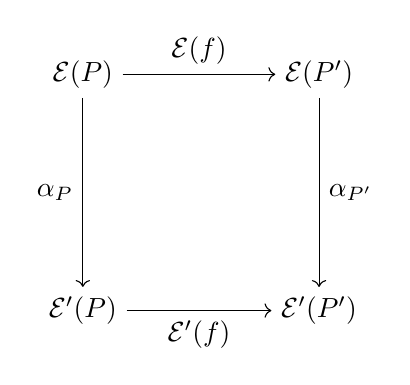
\begin{tikzpicture}[node distance=3cm]
    \node (EP) {$\mathcal{E}(P)$};
    \node (EPP) [right of=EP] {$\mathcal{E}(P')$};
    \node (EPa) [below of=EP] {$\mathcal{E}'(P)$};
    \node (EPPa) [right of=EPa] {$\mathcal{E}'(P')$};

    \draw[->] (EP) -- node[above] {$\mathcal{E}(f)$} (EPP);
    \draw[->] (EP) -- node[left] {$\alpha_P$} (EPa);
    \draw[->] (EPP) -- node[right] {$\alpha_{P'}$} (EPPa);
    \draw[->] (EPa) -- node[below] {$\mathcal{E}'(f)$} (EPPa);
  \end{tikzpicture}
\]

\FigureCallout{Attestations as Natural Transformations (Provenance Commutativity)}{
  The naturality of $\alpha$ ensures that the act of attesting
  ($\alpha_P$) commutes with the act of transforming the payload
  ($\mathcal{E}(f)$).
  This formalizes the requirement that provenance chains remain consistent:
  an attestation applied before or after an update must yield envelopes
  related in a predictable, structure-preserving manner.
}

This formalizes CEP's design principle that attestations do not break
transformations and transformations do not invalidate attestations.

% ------------------------------------------------------------
\subsection{Revision Monotonicity as a Functorial Constraint}
% ------------------------------------------------------------

Let $(\mathbb{N}, \le)$ denote the natural numbers ordered by the usual
non-decreasing relation.
Revision numbers in CEP form a functor:
\[
  \mathrm{Rev} : \mathbf{E} \to (\mathbb{N}, \le),
\]
which assigns to each enveloped record its revision number and to each
morphism $R \to R'$ the corresponding order-preserving mapping
$\mathrm{Rev}(R) \le \mathrm{Rev}(R')$.

Thus, revision monotonicity is not merely a rule but a categorical
invariant: all CEP morphisms must map to monotone arrows in
$(\mathbb{N}, \le)$.
This captures the immutability and forward-only
progression of the revision field as a semantic constraint enforced at
the categorical level.

% ------------------------------------------------------------
\subsection{Envelopes as a Comonad}
% ------------------------------------------------------------

The enveloping process admits an alternative and illuminating
interpretation:
it behaves comonadically when viewed as a context
constructor on payloads~\citep{maclane1971categories,awodey2010category}.

Concretely, consider a category $\mathbf{P}_{\mathsf{env}}$ whose
objects are payloads together with their envelopes, but where we
regard the payload component as primary and the envelope as context.
On this category, an endofunctor
\[
  \mathsf{C} : \mathbf{P}_{\mathsf{env}} \to \mathbf{P}_{\mathsf{env}}
\]
can be defined that ``adds context'' in the sense of enriching a record
with its envelope structure.

A comonad $(\mathsf{C}, \varepsilon, \delta)$ consists of:
\begin{itemize}
  \item a functor $\mathsf{C} : \mathbf{P}_{\mathsf{env}} \to \mathbf{P}_{\mathsf{env}}$,
  \item a counit $\varepsilon : \mathsf{C} \Rightarrow \mathrm{Id}$,
  \item a comultiplication
        $\delta : \mathsf{C} \Rightarrow \mathsf{C}\mathsf{C}$,
\end{itemize}
satisfying standard coassociativity and counitality laws.

In CEP:
\begin{itemize}
  \item $\mathsf{C}(P)$ is the ``contextualized'' version of $P$,
        carrying its envelope,
  \item $\varepsilon$ extracts the underlying payload from its envelope,
  \item $\delta$ enriches a record with its own envelope again,
        representing recursive contextualization (e.g., envelopes of envelopes).
\end{itemize}

This perspective aligns CEP envelopes with the comonadic
interpretation of contextual data in database theory~\citep{spivak2014category}.

% ------------------------------------------------------------
\subsection{Attestations as a Cartesian Natural Transformation}
% ------------------------------------------------------------

Not all natural transformations preserve the limit structure needed for
record-level consistency.
CEP attestations must preserve pullbacks:
they cannot break joins or invalidate prior provenance.

Thus we refine $\alpha : \mathcal{E} \Rightarrow \mathcal{E}'$ to be a
\emph{cartesian natural transformation}, meaning that each naturality
square is a pullback square.

Formally, for every $f : P \to P'$,
\[
  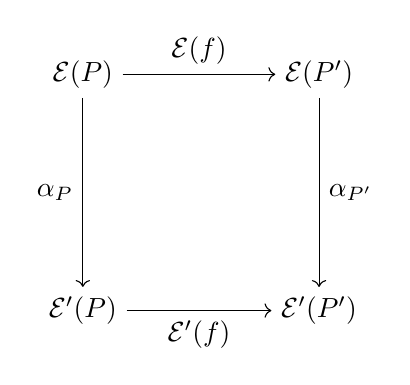
\begin{tikzpicture}[node distance=3cm]
    \node (EP) {$\mathcal{E}(P)$};
    \node (EPP) [right of=EP] {$\mathcal{E}(P')$};
    \node (EPa) [below of=EP] {$\mathcal{E}'(P)$};
    \node (EPPa) [right of=EPa] {$\mathcal{E}'(P')$};

    \draw[->] (EP) -- node[above] {$\mathcal{E}(f)$} (EPP);
    \draw[->] (EP) -- node[left] {$\alpha_P$} (EPa);
    \draw[->] (EPP) -- node[right] {$\alpha_{P'}$} (EPPa);
    \draw[->] (EPa) -- node[below] {$\mathcal{E}'(f)$} (EPPa);
  \end{tikzpicture}
\]
is required to be a pullback.

Cartesianness ensures:
\begin{itemize}
  \item attestations preserve joins,
  \item no new contradictions arise under $\alpha$,
  \item provenance behaves consistently across merges.
\end{itemize}

This matches CEP's requirement that attestations cannot ``detach'' from
the record state they certify.

% ------------------------------------------------------------
\subsection{CEP as a Fibred Category}
% ------------------------------------------------------------

Let $\mathbf{Sch}$ denote the category of CEP schemas and controlled
vocabulary URIs.
Each CEP record is typed by a schema element, giving rise to a functor:
\[
  \pi : \mathbf{CEP} \to \mathbf{Sch}.
\]

We interpret $\pi$ as a \emph{fibration}: for any morphism
$s : S \to S'$ in $\mathbf{Sch}$ and any record $R'$ over $S'$, there
exists a \emph{cartesian lifting} describing the induced transformation
on record instances.

This validates two core CEP invariants:
\begin{itemize}
  \item type-consistent updates always exist,
  \item vocabulary and schema evolution propagate along cartesian liftings.
\end{itemize}

The fibred structure provides the mathematical foundation for version
migration and schema evolution.

% ------------------------------------------------------------
\subsection{Relation to W3C PROV}
% ------------------------------------------------------------


CEP attestation components align directly with PROV-DM constructs:
\begin{center}
  \begin{tabular}{ll}
    \toprule
    CEP Component                 & PROV Construct                                      \\
    \midrule
    \texttt{attestorId}           & \texttt{prov:Agent}                                 \\
    \texttt{attestationTimestamp} & \texttt{prov:Generation} / \texttt{prov:Start}      \\
    \texttt{proofType}            & \texttt{prov:Activity} type                         \\
    \texttt{proofPurpose}         & \texttt{prov:Plan} or \texttt{prov:Role}            \\
    \texttt{proofValue}           & \texttt{prov:Entity} / \texttt{prov:wasGeneratedBy} \\
    \bottomrule
  \end{tabular}
\end{center}

Categorically, PROV's \texttt{wasGeneratedBy} and \texttt{wasAttributedTo}
become morphisms in a provenance category $\mathbf{Prov}$.
The attestation natural transformation $\alpha$ factors through a functor:
\[
  A : \mathbf{CEP} \to \mathbf{Prov},
\]
thereby embedding CEP provenance into the PROV lineage.

This establishes a formal bridge between CEP's categorical semantics
and the W3C PROV standard for provenance representation.
          % Natural Transformations (Envelopes, Attestations)
% !TeX root = 00_cep_semantics.tex

\section{Canonicalization as a Monoidal Functor}
\label{sec:canonicalization}

Canonicalization is the mathematical process that ensures the stability
and uniqueness of the SNFEI identifier.
In the Civic Exchange Protocol (CEP), normalization and assembly are
expressed as a structured rewriting system and modeled categorically
as a composite of functors equipped with
a strict monoidal structure.

% ----------------------------------------------------------------------
\paragraph{Ordering of Rewrite Rules.}

We regard normalization as a total function
\[
  \mathrm{norm} : \mathrm{RawString} \to \mathrm{CanonicalString}.
\]
Rewrite operations occur at three levels: (1)~semantic expansions,
(2)~structural simplifications, and (3)~surface-level normalizations.
Some rewrites preserve information while others reduce it, so their order
is essential.
For example, the corporate form ``S.A.'' must be expanded
before punctuation is removed; otherwise the pattern disappears and the
expansion cannot apply.

CEP adopts a \emph{stratified} rewriting system with a fixed ordering of
rule strata.
Rewrite rules compose associatively within each stratum.
Across strata, the ordering is not assumed to commute and is treated as
part of the definition of the normalization pipeline.

This behavior is representative rather than exceptional: whenever a
semantic rewrite depends on surface structure, rewrite order becomes
semantically meaningful and cannot be treated as commutative.


% ----------------------------------------------------------------------
\subsubsection{Stratified Canonicalization as a Functor}

Let $\Raw$ be the set of raw strings and $\Canon$ the set of canonical
forms, viewed as a quotient of $\Raw$ under an equivalence relation that
identifies strings representing the same civic entity.
Let
\[
  q : \Raw \to \Canon
\]
be the quotient map selecting canonical representatives.

Normalization is implemented by a finite sequence of rewrite functions
\[
  n_1, n_2, \dots, n_k : \Raw \to \Raw,
\]
each belonging to a particular stratum.
Within a stratum composition is
associative; across strata the evaluation order is fixed.
The overall normalization map is
\[
  \mathrm{norm}
  \;=\;
  q \circ n_k \circ \dots \circ n_2 \circ n_1
  : \Raw \to \Canon.
\]

Categorically, each $n_i$ is an endomorphism of $\Raw$ in $\mathbf{Set}$.
The rule strata form a thin (preordered) category $\mathcal{S}$.
The normalization pipeline is a functor
\[
  F : \mathcal{S} \to \mathbf{End}(\Raw),
\]
where $\mathbf{End}(\Raw)$ is the monoidal category of endofunctions on
$\Raw$ under composition.
The fixed order of $\mathcal{S}$ determines the
evaluation of the composite; commutativity is not required.

% ----------------------------------------------------------------------
\paragraph{Diagrammatic View.}

\[
  \begin{tikzcd}
    \Raw \arrow[r, "n_1"]
    \arrow[rr, bend left=30, "n_2 \circ n_1"]
    \arrow[rrr, bend left=45, "n_3 \circ n_2 \circ n_1"]
    &
    \Raw \arrow[r, "n_2"]
    &
    \Raw \arrow[r, "n_3"]
    &
    \Raw \arrow[r, "q"]
    &
    \Canon
  \end{tikzcd}
\]

Associativity of composition gives
\[
  (n_3 \circ n_2) \circ n_1 = n_3 \circ (n_2 \circ n_1),
  \qquad
  \mathrm{norm} = q \circ n_3 \circ n_2 \circ n_1.
\]
Stratification appears as the requirement that the arrows $n_i$ occur in a
fixed left-to-right order.

% ----------------------------------------------------------------------
\paragraph{Relation to Rewriting Systems.}

Many established rewriting systems use ordered or strategy-driven rule
application.
Classical completion procedures, modern term-rewriting
frameworks, compiler pipelines, natural-language normalization workflows,
and Unicode normalization all apply structured, multi-stage rewriting in
which information-preserving rewrites precede information-reducing ones.

CEP follows this standard pattern.
Each stratum contains rewrite rules that compose cleanly within their domain,
while the fixed ordering across strata functions as the evaluation strategy
that guarantees determinism of the composite normalization function.

This strategy-controlled evaluation means that CEP canonicalization is not
intended to be confluent or transitive with respect to individual rewrite rules.
Only the fully evaluated composite function norm defines the canonical equivalence
relation.

% ----------------------------------------------------------------------
\subsubsection{Rewriting Systems as 2-Categories}

Rewriting systems may be described in terms of 2-categories or polygraphs:
objects are syntactic states, 1-morphisms are rewrite steps, and
2-morphisms represent coherence between rewrite paths.
Normalization corresponds to selecting a distinguished representative of each connected
component of the 1-skeleton.

CEP fits this model.
Each stratum consists of 1-morphisms that are closed
under associative composition, while the ordering of strata specifies a
deterministic rewriting strategy.
The normalization map
\[
  \mathrm{norm} : \Raw \to \Canon
\]
is therefore a strategy-controlled composite followed by quotienting.

% ======================================================================
\subsection{The Normalizing Functor
  \texorpdfstring{$\mathcal{F}_{\mathrm{normalize}}$}{F\_normalize}}
% ======================================================================

Let $\mathbf{R}_{\text{raw}}$ be the category whose objects are raw
record states and whose morphisms are valid transformations between them.
Let $\mathbf{R}_{\text{canon}}$ be the corresponding category of
canonical states.

Normalization is a functor
\begin{equation}
  \mathcal{F}_{\mathrm{normalize}} :
  \mathbf{R}_{\text{raw}} \to \mathbf{R}_{\text{canon}}.
\end{equation}

For any morphism $f : R \to R'$ in $\mathbf{R}_{\text{raw}}$, functoriality
ensures that
\[
  \mathcal{F}_{\mathrm{normalize}}(f) :
  \mathcal{F}_{\mathrm{normalize}}(R)
  \to
  \mathcal{F}_{\mathrm{normalize}}(R')
\]
is the corresponding update on canonical records.

% ======================================================================
\subsection{Monoidal Structure and the Canonicalization Functor
  \texorpdfstring{$\mathcal{C}$}{C}}
% ======================================================================

Let $\mathbf{R}_{\text{canon}}$ carry a monoidal structure in which
objects represent normalized components and $\otimes$ denotes their
ordered concatenation.
Let $\mathbf{C}$ be the category of canonical strings with monoidal product
also given by concatenation and unit $I$.

The assembly step is a strict monoidal functor
\begin{equation}
  \mathcal{C} : (\mathbf{R}_{\text{canon}}, \otimes, I)
  \to (\mathbf{C}, \otimes, I)
\end{equation}
satisfying
\begin{equation}
  \mathcal{C}(x \otimes y) = \mathcal{C}(x) \otimes \mathcal{C}(y),
  \qquad
  \mathcal{C}(I) = I.
\end{equation}

This functor performs the disciplined concatenation that assembles
canonical parts (name, address, date, jurisdiction) into a single string
in the fixed order prescribed by CEP.

% ======================================================================
\subsection{From Canonical Strings to SNFEI}
% ======================================================================

Let
\[
  H : \mathbf{C} \to \mathbf{ID}
\]
be the hashing functor that maps canonical strings to 256-bit identifiers
via the SHA-256 cryptographic hash function.
For a record $R$,
\[
  \mathrm{SNFEI}(R)
  =
  H\!\left(\mathcal{C}(R_{\text{canon}})\right),
  \qquad
  R_{\text{canon}} =
  \mathcal{F}_{\mathrm{normalize}}(R_{\text{raw}}).
\]

The full pipeline is the composite functor
\begin{equation}
  H \circ \mathcal{C} \circ \mathcal{F}_{\mathrm{normalize}}
  : \mathbf{R}_{\text{raw}} \to \mathbf{ID}.
\end{equation}

\begin{figure}[ht]
  \centering
  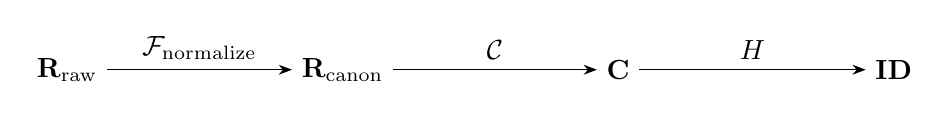
\begin{tikzpicture}[node distance=3.5cm,>=Stealth]
    \node (raw)   {$\mathbf{R}_{\text{raw}}$};
    \node (canon) [right of=raw] {$\mathbf{R}_{\text{canon}}$};
    \node (C)     [right of=canon] {$\mathbf{C}$};
    \node (id)    [right of=C] {$\mathbf{ID}$};

    \draw[->] (raw)   -- node[above]
    {$\mathcal{F}_{\mathrm{normalize}}$} (canon);
    \draw[->] (canon) -- node[above]
    {$\mathcal{C}$} (C);
    \draw[->] (C)     -- node[above]
    {$H$} (id);
  \end{tikzpicture}
  \caption{Canonicalization pipeline from raw records to stable identifiers.}
  \label{fig:canonicalization-pipeline}
\end{figure}

% ======================================================================
\subsection{Identifier Invariance and Equivalence Classes}
% ======================================================================

\textbf{Invariance Principle.}
If $f : R \to R'$ is an identity-preserving morphism in the category
$\mathbf{CEP}$ of valid CEP record states and updates, then
\[
  H \circ \mathcal{C} \circ \mathcal{F}_{\mathrm{normalize}}(R)
  =
  H \circ \mathcal{C} \circ \mathcal{F}_{\mathrm{normalize}}(R').
\]

Identity-preserving updates therefore do not change the SNFEI.
Two record states lie in the same equivalence class precisely when they produce the
same canonical string and hence the same identifier.
Strict monoidality of $\mathcal{C}$ ensures that required components appear in the correct
order and cannot be reordered or omitted along valid CEP morphisms.

\FigureCallout{Canonicalization as a Monoidal Functor and Identity Guarantee}{
  Because $\mathcal{F}_{\mathrm{normalize}}$ and $\mathcal{C}$ are
  functorial, and $\mathcal{C}$ is strictly monoidal, the canonical string
  associated with an entity is uniquely determined by its
  identity-bearing fields.
  The SNFEI is therefore a function of an equivalence class of records
  rather than any particular representation.}

This invariance principle underpins CEP's claims of stable,
provenance-respecting identifiers suitable for cross-jurisdiction
linkage and data fusion.   % Canonicalization as Strict Monoidal Functor
% ============================================================
\section{Jurisdictional Adapters as Oplax Functors}
\label{sec:adapters}
% ============================================================

\subsection{Motivation}

Jurisdictions frequently maintain their own data schemas, codes, or
structural conventions. Let $\mathbf{J_{\mathrm{local}}}$ denote the
category generated by a jurisdiction's native schema and transformation
rules, and let $\mathbf{J_{\mathrm{global}}}$ denote the category
induced by CEP vocabularies and canonical record structures.

Any adapter must reconcile these two perspectives. However, the mapping
from local to global structure is typically \emph{weak}: optional fields
may not appear locally, local compositions may collapse distinctions
preserved globally, and some structural information may be lost.

This motivates the use of \emph{oplax functors}, which formalize
structure-weakening translations between categories.

% ------------------------------------------------------------
\subsection{Oplax Functor
  \texorpdfstring{$\mathcal{A}$}{A}}
% ------------------------------------------------------------

An adapter is modeled as an oplax functor
\begin{equation}
  \mathcal{A} :
  \mathbf{J_{\mathrm{local}}}
  \longrightarrow
  \mathbf{J_{\mathrm{global}}}.
\end{equation}

For every pair of composable morphisms
$f : X \to Y$ and $g : Y \to Z$ in
$\mathbf{J_{\mathrm{local}}}$, oplaxity means that we have a
\emph{coherence morphism}
\begin{equation}
  \phi_{f,g} :
  \mathcal{A}(g) \circ \mathcal{A}(f)
  \;\Longrightarrow\;
  \mathcal{A}(g \circ f),
\end{equation}
which need not be invertible. This captures the possibility of
\emph{lossy harmonization}: two distinct local transformations may be
indistinguishable at the global level.

\begin{figure}[h]
  \centering
  \begin{tikzpicture}[node distance=3.2cm,>=Stealth]
    \node (X) {$X$};
    \node (Y) [right of=X] {$Y$};
    \node (Z) [right of=Y] {$Z$};

    \draw[->] (X) -- node[above] {$f$} (Y);
    \draw[->] (Y) -- node[above] {$g$} (Z);

    \node (AX) [below of=X, yshift=-1.2cm] {$\mathcal{A}(X)$};
    \node (AY) [below of=Y, yshift=-1.2cm] {$\mathcal{A}(Y)$};
    \node (AZ) [below of=Z, yshift=-1.2cm] {$\mathcal{A}(Z)$};

    \draw[->] (AX) -- node[above] {$\mathcal{A}(f)$} (AY);
    \draw[->] (AY) -- node[above] {$\mathcal{A}(g)$} (AZ);

    \draw[->, dashed, bend left=35]
      (AX) to node[below] {$\mathcal{A}(g \circ f)$} (AZ);

    \draw[->, shorten >=6pt, shorten <=6pt]
      ($(AY)!0.5!(AZ)$) -- node[right] {$\phi_{f,g}$}
      ($(AX)!0.5!(AY)$);
  \end{tikzpicture}
  \caption{An oplax adapter: compositions are preserved only up to a
    coherence morphism $\phi_{f,g}$.}
  \label{fig:oplax-adapter}
\end{figure}

This structure formalizes \textbf{Jurisdictional Autonomy}:  
local schemas may preserve distinctions or collapse details not present
in the global vocabulary, while still participating coherently in the
CEP ecosystem.

\FigureCallout{Adapters as Oplax Functors (Jurisdictional Autonomy)}{
An oplax functor models the fact that the translation from a local
schema to the global CEP vocabulary may weaken structure. Local
compositions $g \circ f$ may only match their global images up to a
coherence morphism $\phi_{f,g}$, reflecting partial, lossy, or
jurisdiction-specific mappings. This accommodates local flexibility
without violating global interoperability.
}

% ------------------------------------------------------------
\subsection{Correctness Criteria for Adapters}
% ------------------------------------------------------------

A jurisdictional adapter $\mathcal{A}$ is valid for CEP if and only if
it satisfies the following criteria:

\begin{enumerate}
  \item \textbf{Required-field preservation.}
    For every required local field,  
    $\mathcal{A}$ must map it to a required term in the CEP vocabulary.
    Formally, required morphisms in $\mathbf{J_{\mathrm{local}}}$
    must map to required morphisms in $\mathbf{J_{\mathrm{global}}}$.

  \item \textbf{Optional weakening via coherence.}
    Optional fields or partial structures must be captured by the oplax
    coherence morphisms $\phi_{f,g}$, ensuring that weakened structure
    is still well-typed globally.

  \item \textbf{Canonicalization compatibility.}
    The canonical identifier must be computable on the image of the
    adapter:
    \begin{equation}
      \mathcal{C}(\mathcal{A}(R))
      \quad \text{is defined for all admissible local records } R.
    \end{equation}
    This guarantees that local jurisdictions can produce stable and
    globally comparable SNFEI identifiers.

  \item \textbf{Provenance monotonicity.}
    Adapter-induced transformations must not contradict envelope
    attestations or revision-order invariants established in
    $\mathbf{CEP}$.

  \item \textbf{Functoriality on valid updates.}
    For any valid local update $u : R \to R'$, the image
    $\mathcal{A}(u)$ must remain a valid update in the CEP record
    system, modulo the required oplax coherence.
\end{enumerate}

A valid adapter therefore acts as a structure-respecting mediator
between local civic systems and the global CEP representation while
allowing precisely the amount of structural weakening necessary for
jurisdictional independence.
           % Jurisdictional Adapters as Oplax Functors
% !TeX root = 00P2_cep_semantics.tex

\section{Context Tags as Indexed Families}
\label{sec:ctags}

\subsection{\texorpdfstring{Fibered Category
    $\pi : \mathbf{CT} \to \mathbf{CEP}$}
  {Fibered Category pi : CT → CEP}}
% ------------------------------------------------------------

Context tags (CTags) are interpretive annotations attached to a record
without altering its canonical identity.
Their semantics is captured by a
\emph{fibered category}
\begin{equation}
  \pi : \mathbf{CT} \longrightarrow \mathbf{CEP},
\end{equation}
where:
\begin{itemize}
  \item $\mathbf{CEP}$ is the base category of identity-bearing records,
  \item $\mathbf{CT}$ consists of pairs $(R, T)$ of a CEP record $R$ and an attached context tag $T$,
  \item $\pi$ is the projection functor $\pi(R, T) = R$.
\end{itemize}

For a base object $R \in \mathbf{CEP}$, the fiber
\[
  \mathbf{CT}_R = \{ (R, T) \in \mathbf{CT} \mid \pi(R,T) = R \}
\]
collects all valid context tags that may be associated with $R$.
These fibers encode analytic or interpretive information while leaving the
canonical structure and identifier of $R$ unchanged.

\FigureCallout{Context Tags in a Fibered Category (Separation of Concerns)}{
  The projection $\pi : \mathbf{CT} \to \mathbf{CEP}$ cleanly separates
  \emph{identity} (records in $\mathbf{CEP}$) from \emph{interpretation}
  (tags in the fibers $\mathbf{CT}_R$).
  Any morphism in $\mathbf{CEP}$
  induces a coherent reindexing across fibers, ensuring that context tags
  evolve with records while never influencing their SNFEI identity.
}

% ------------------------------------------------------------
\subsection{Functoriality and Reindexing}
% ------------------------------------------------------------

Let
\[
  f : R \longrightarrow R'
\]
be a morphism in $\mathbf{CEP}$ representing a valid evolution or update
of a record.
The fibration provides a corresponding \emph{reindexing
  functor}
\begin{equation}
  f^\ast : \mathbf{CT}_{R'} \longrightarrow \mathbf{CT}_R.
\end{equation}

Intuitively, $f^\ast$ specifies how tags attached to the updated record
$R'$ may be pulled back to valid tags on the earlier state $R$,
preserving interpretive meaning along the update path.

\begin{figure}[ht]
  \centering
  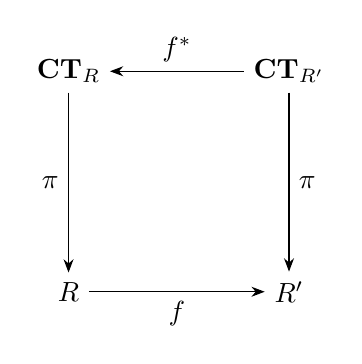
\begin{tikzpicture}[node distance=2.8cm,>=Stealth]
    \node (CR) {$\mathbf{CT}_R$};
    \node (CRp) [right of=CR] {$\mathbf{CT}_{R'}$};

    \node (R) [below of=CR] {$R$};
    \node (Rp) [below of=CRp] {$R'$};

    \draw[->] (CRp) -- node[above] {$f^\ast$} (CR);
    \draw[->] (R) -- node[below] {$f$} (Rp);

    \draw[->] (CR) -- node[left] {$\pi$} (R);
    \draw[->] (CRp) -- node[right] {$\pi$} (Rp);
  \end{tikzpicture}
  \caption{Reindexing in the fibration $\pi : \mathbf{CT} \to \mathbf{CEP}$.}
  \label{fig:fibration-reindex}
\end{figure}

Reindexing satisfies the standard fibration condition:
\begin{equation}
  \pi \circ f^\ast = f \circ \pi,
\end{equation}
so the diagram in Figure~\ref{fig:fibration-reindex} commutes.
Thisexpresses the guiding CEP principle:

\begin{quote}
  \textbf{Context tags move with the record's evolution but never change
    its identity.}
\end{quote}

% ------------------------------------------------------------
\subsection{Identity Preservation and Canonical Invariance}
% ------------------------------------------------------------

A tag object $T \in \mathbf{CT}_R$ must not modify any canonical data
used in identifier generation.
Formally, if $\mathcal{C}$ denotes thecanonicalization functor, then
\begin{equation}
  \mathcal{C}(R) = \mathcal{C}(R, T),
\end{equation}
so attaching tags does not affect the canonical form of $R$.

Equivalently, the projection functor $\pi$ is \emph{identity-reflecting}:
if two tagged objects $(R,T)$ and $(R',T')$
yield the same canonical identifier,
then $R$ and $R'$ must already be
identified in the base category $\mathbf{CEP}$.

Consequently:
\begin{itemize}
  \item CTags are \emph{pure annotations};
  \item they introduce no new canonical structure;
  \item they cannot alter SNFEI values or canonical equivalence classes.
\end{itemize}

This establishes a strict separation between
\[
  \text{identity} \quad (\mathbf{CEP})
  \qquad\text{and}\qquad
  \text{interpretation} \quad (\mathbf{CT}_R).
\]
\FigureCallout{Identity Preservation via Context Tags}{
  Context tags in the fibered category $\pi : \mathbf{CT} \to \mathbf{CEP}$
  are strictly non-influential on canonical identity. The projection
  $\pi$ ensures that no tagged object $(R,T)$ can alter the canonical form
  or SNFEI of its base record $R$, preserving CEP's invariants.
}
              % Context Tags as Fibration
% !TeX root = 00P2_cep_semantics.tex

\section{Interoperability Results}
\label{sec:results}

The categorical semantics developed in the preceding sections yield
formal guarantees for CEP's core interoperability claims.
These results follow from functoriality, naturality, monoidal structure, and the oplax
semantics of jurisdictional adapters.
All results are stated relative to the category $\mathbf{CEP}$ and
therefore apply only to admissible record states and total,
invariant-preserving transformations.

% ------------------------------------------------------------
\subsection{Functorial Consistency}
% ------------------------------------------------------------

We first establish coherence between record evolution and attestation.

\begin{lemma}[Functorial Consistency of Attested Evolutions]
  \label{lemma:functorial-consistency}
  Let $f : R \to R'$ and $g : R' \to R''$ be morphisms in
  $\mathbf{CEP}$, and let $\alpha : \mathcal{E} \Rightarrow \mathcal{E}'$
  be the natural transformation representing attestation.
  Then:
  \[
    \mathcal{E}'(g \circ f)
    \;=\;
    \alpha_{R''} \circ \mathcal{E}(g \circ f)
    \;=\;
    \mathcal{E}'(g) \circ \mathcal{E}'(f).
  \]
\end{lemma}

\begin{proof}
  Naturality of $\alpha$ gives
  \(
  \alpha_{R'} \circ \mathcal{E}(f)
  =
  \mathcal{E}'(f) \circ \alpha_R
  \)
  for all $f : R \to R'$.
  Composing these constraints and using associativity
  of morphisms in $\mathbf{CEP}$ yields the claim.
\end{proof}

This shows that CEP's update--attestation workflow behaves coherently
under composition, supporting reliable audit chains and immutability of
provenance traces.

% ------------------------------------------------------------
\subsection{Identifier Preservation}
% ------------------------------------------------------------

We now formalize the stability of canonical identifiers under all valid
record evolutions.

\begin{theorem}[Identifier Preservation]
  \label{thm:identifier-preservation}
  Let $f : R \to R'$ be any morphism in $\mathbf{CEP}$.
  Let $\mathcal{C}$
  denote the canonicalization functor and
  $H$ the deterministic hash used to compute the SNFEI.
  Then:
  \[
    H(\mathcal{C}(R)) \;=\; H(\mathcal{C}(R')).
  \]
\end{theorem}

\begin{proof}
  A valid $\mathbf{CEP}$ morphism $f$ preserves all canonical components
  of the record.
  Strict monoidality of $\mathcal{C}$ therefore implies
  $\mathcal{C}(R)=\mathcal{C}(R')$.
  Since $H$ is a pure function, the
  resulting SNFEI values coincide.
\end{proof}

This theorem provides the mathematical foundation for CEP's claim of
\emph{identity stability across revisions}.

% ------------------------------------------------------------
\subsection{Cross-Jurisdiction Reconciliation}
% ------------------------------------------------------------

Jurisdictional adapters reconcile heterogeneous local schemas with the
global CEP vocabulary.
We show that their oplax semantics preserves canonical identity across compositions.

\begin{theorem}[Canonical Equivalence Preservation Under Adapters]
  \label{thm:adapter-preservation}
  Let $\mathcal{A}_1$ and $\mathcal{A}_2$ be valid jurisdictional
  adapters (Section~\ref{sec:adapters}).
  If two local records $R$ and $R'$ satisfy
  \[
    H(\mathcal{C}(\mathcal{A}_1(R)))
    \;=\;
    H(\mathcal{C}(\mathcal{A}_1(R'))),
  \]
  then after composition with a second adapter,
  \[
    H(\mathcal{C}(\mathcal{A}_2(\mathcal{A}_1(R))))
    \;=\;
    H(\mathcal{C}(\mathcal{A}_2(\mathcal{A}_1(R')))).
  \]
\end{theorem}

\begin{proof}
  A valid adapter is oplax: it may weaken structure but cannot introduce
  new canonical content.
  Thus each $\mathcal{C}(\mathcal{A}_i(R))$ is defined and
  invariant under further valid transformations.
  Strict monoidality of $\mathcal{C}$ ensures that canonical strings are
  preserved under composition of such structure-weakening functors.
  Applying $H$ yields the result.
\end{proof}

\noindent
This theorem shows that multi-stage, cross-jurisdiction pipelines respect
CEP's canonical identity invariants.
It provides the formal backbone for
\emph{globally consistent, locally autonomous interoperability}.
            % Correctness Results
% !TeX root = 00_cep_semantics.tex

\section{Applications}
\label{sec:apps}

The categorical semantics developed above manifest directly in real civic
data workflows.
Domain schemas provide typed structures for entities and exchanges,
while CEP vocabularies furnish the controlled classifications
and relationship types used throughout these workflows.
The following examples illustrate how functoriality, monoidality, pullbacks,
and oplax adapter semantics enforce CEP's core invariants in practice.

% ------------------------------------------------------------
\subsection{Civic Entity Records: Identity Stability}
% ------------------------------------------------------------

Every domain schema (e.g., municipal, educational, environmental) defines
a category of entity revisions whose morphisms correspond to admissible
updates.
A municipal entity's lifecycle is therefore a chain in
$\mathbf{CEP}$:
\[
  E_1 \xrightarrow{f_1} E_2 \xrightarrow{f_2} \cdots
\]
where each $E_i$ conforms to the relevant domain schema and vocabulary.

Identity Invariance ensures that any identity-preserving update $f_i$
leaves the canonical form unchanged:
\[
  \mathcal{C}(E_i) = \mathcal{C}(E_{i+1}).
\]
Thus the SNFEI remains stable even as auxiliary fields (address,
classification, jurisdictional codes, vocabulary-driven status fields)
evolve over time.
The vocabulary layer guarantees that enumerated fields
(e.g.\ \texttt{ACTIVE}, \texttt{DISSOLVED}) remain consistent across
revisions and jurisdictions.

This yields a strong operational principle:

\begin{quote}
  \textbf{Domain schemas define the structure of change; canonicalization
    guarantees that such change never affects identity.}
\end{quote}

% ------------------------------------------------------------
\subsection{Campaign Finance: Compositional Provenance}
% ------------------------------------------------------------

Domain schemas for campaign finance define typed exchange morphisms,
where controlled vocabulary terms specify the semantics of each transfer
(e.g.\ \texttt{donation}, \texttt{in-kind}, \texttt{reallocation}).

A donation from a donor $D$ to a committee $C$ is a morphism
$f : D \to C$.
A downstream transfer from $C$ to a subcommittee $S$ is
a morphism $g : C \to S$.
Their composition
\[
  g \circ f : D \to S
\]
represents the derived provenance lineage.

Because composition in $\mathbf{CEP}$ is associative and is compatible with the vocabulary-governed domain schema,
this lineage is canonical across all reporting systems.
It enables coherent financial traceability even
when jurisdictions differ in local reporting conventions—oplax adapters
(Section~\ref{sec:adapters}) ensure that structure-weakening translations
still preserve this compositional provenance.

% ------------------------------------------------------------
\subsection{Public Contracting: Data Fusion via Pullbacks}
% ------------------------------------------------------------

Public contracting data arises from multiple domain schemas:
\begin{itemize}
  \item Vendor Registry schema (legal entities, certifications, status),
  \item Contract schema (awards, amendments, payments),
  \item Jurisdiction-specific extensions and vocabularies.
\end{itemize}

Suppose a Vendor Registry record $R_V$ and a Contract Record $R_C$ both
reference the same underlying legal entity $A$.
The fiber product
\[
  P = R_V \times_A R_C
\]
constructs the maximal consistent set of jointly satisfiable facts.
This pullback operation merges information along the shared canonical identity
specified by the SNFEI and vocabulary-controlled relationship types.

This is the categorical mechanism that guarantees sound cross-system
integration.
It ensures that:

\begin{itemize}
  \item canonical identity aligns disparate domain schemas,
  \item vocabulary-governed code systems reconcile classification fields,
  \item provenance constraints remain intact across fused datasets.
\end{itemize}

As a result, auditors can reconcile procurement data across heterogeneous
jurisdictional sources, even when local schemas differ substantially, while
maintaining CEP's global invariants.

               % Applications and Use Cases
% !TeX root = 00P2_cep_semantics.tex


\section{Limitations and Future Work}
\label{sec:limitations}

The categorical core presented in this paper captures identity,
canonicalization, provenance, and interoperability for discrete,
revision-based civic records.
Several important extensions remain outside the present scope.

Many civic systems also generate data that is statistical, uncertain, or
continuously updated (e.g., longitudinal indicators, evolving aggregates).
Incorporating such information may require probabilistic semantics or
temporal indexing, which are not modeled in the current framework.

Jurisdictions evolve data models over time.
Although CEP supports adapters for structural variation,
a full account of schema evolution, including additions,
deprecations, and long-term migration paths, remains future work.

\paragraph{Multi-Stage and Nested Exchanges.}

Some workflows involve layered or multi-party processes
(e.g., multi-level budget allocations, nested reporting pipelines).
These may benefit from higher-structured categorical tools,
but such extensions lie beyond the scope of this foundational treatment.

\paragraph{Rule Sensitivity in Canonicalization.}

Certain linguistic cases (such as expansions of abbreviations like “S.A.”)
require stratified rule ordering within the normalization pipeline rather
than treating all rewrite rules as freely permutable.
This refinement does not affect the well-definedness of the canonicalization
function but does highlight the need for continued empirical tuning of rule strata.

\medskip

The present semantics establish a robust core for identity and interoperability.
Extending CEP to the richer data practices found across governments and civic ecosystems
is a key direction for future work.

% ------------------------------------------------------------
\section{Conclusion}
\label{sec:conclusion}

We presented a categorical semantics for the Civic Exchange Protocol
that unifies canonicalization, provenance, adapters, and context tags
into a coherent mathematical framework.
This perspective makes explicit the invariants that govern identity,
record evolution, and interoperability across heterogeneous civic data systems.

Canonicalization was formulated as a deterministic monoidal functor,
ensuring stable identifiers and well-defined equivalence classes.
Jurisdictional adapters were modeled as oplax functors, capturing how
local structure may be weakened while preserving global identity.
Context tags were expressed via a fibered category, isolating
interpretive annotations from canonical record content.
Together, these structures yield formal guarantees for identifier preservation,
compositional provenance, and cross-jurisdiction reconciliation.

The resulting semantics provides a rigorous foundation for validation,
verification, and future extensions of CEP.
It enables principled design of domain schemas, vocabularies,
and interoperability standards, while remaining extensible to evolving civic workflows.
As civic data ecosystems continue to grow in scale and complexity,
categorical methods offer a durable and expressive language for ensuring that shared
identities and exchanges remain consistent, transparent, and reliable.


\section*{Acknowledgements}

Portions of this work were developed through human-computer collaboration
using modern computational tools.
Generative language models were used to assist with editing, formatting,
and consistency checking during manuscript preparation.
All conceptual framing, formal development, results, interpretations, and conclusions
are the author's own.
All generated suggestions were critically reviewed and validated, and
the author takes full responsibility for the content of this work.         % Limitations, Future Work, Conclusion

\appendix
\clearpage

% ============================================================
\appendix
\section*{Appendix A. Category-Theoretic Background}
\addcontentsline{toc}{section}{Appendix A. Category-Theoretic Background}
% ============================================================

This appendix summarizes the categorical notions used in the paper.
It is intended for readers with a background in data modeling,
databases, or formal methods who may not use category theory daily.
The goal is conceptual clarity rather than mathematical depth.

% ------------------------------------------------------------
\subsection*{A.1 Categories}
% ------------------------------------------------------------

A \emph{category} consists of:
\begin{itemize}
    \item a collection of \textbf{objects};
    \item a collection of \textbf{morphisms} (arrows) between objects;
    \item an associative composition operation
          and an identity arrow for each object.
\end{itemize}

Intuition:
\begin{itemize}
    \item Objects represent states or structured data (e.g., CEP records).
    \item Morphisms represent valid transformations (e.g., amendments).
    \item Composition corresponds to applying transformations sequentially.
\end{itemize}

\medskip
Example:
A sequence of record updates in CEP corresponds to a chain of morphisms
\[ R_0 \to R_1 \to R_2 \to \cdots. \]

% ------------------------------------------------------------
\subsection*{A.2 Functors}
% ------------------------------------------------------------

A \emph{functor} $F : \mathbf{C} \to \mathbf{D}$ maps:
\begin{itemize}
    \item each object of $\mathbf{C}$ to an object of $\mathbf{D}$,
    \item each morphism in $\mathbf{C}$ to a morphism in $\mathbf{D}$,
\end{itemize}
such that identities and composition are preserved.

Intuition:
\begin{itemize}
    \item A functor is a structure-preserving translation.
    \item CEP uses functors to model processes such as
          envelope construction or canonicalization.
\end{itemize}

% ------------------------------------------------------------
\subsection*{A.3 Natural Transformations}
% ------------------------------------------------------------

Given functors $F, G : \mathbf{C} \to \mathbf{D}$,
a \emph{natural transformation} $\eta : F \Rightarrow G$ assigns
to each object $X$ in $\mathbf{C}$ a morphism
\[
\eta_X : F(X) \to G(X)
\]
such that each square
\[
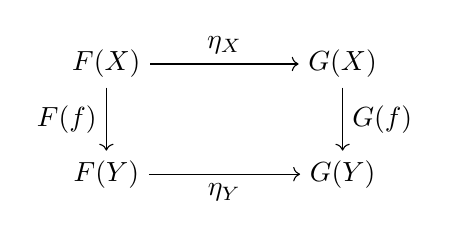
\begin{tikzpicture}[baseline=(current bounding box.center)]
\node (FX) at (0,0) {$F(X)$};
\node (GX) at (3,0) {$G(X)$};
\node (FY) at (0,-1.4) {$F(Y)$};
\node (GY) at (3,-1.4) {$G(Y)$};
\draw[->] (FX) -- node[above] {$\eta_X$} (GX);
\draw[->] (FY) -- node[below] {$\eta_Y$} (GY);
\draw[->] (FX) -- node[left] {$F(f)$} (FY);
\draw[->] (GX) -- node[right] {$G(f)$} (GY);
\end{tikzpicture}
\]
commutes for all morphisms $f : X \to Y$.

Intuition:
\begin{itemize}
    \item Naturality means: \emph{"attest first then transform" =
          "transform first then attest"}. 
    \item This is exactly the coherence needed for CEP attestation chains.
\end{itemize}

% ------------------------------------------------------------
\subsection*{A.4 Monoidal Categories}
% ------------------------------------------------------------

A \emph{monoidal category} is a category equipped with:
\begin{itemize}
    \item a tensor product $\otimes$ combining objects,
    \item a unit object $I$,
    \item coherence laws ensuring associativity and proper unit behavior.
\end{itemize}

In CEP, the relevant monoidal structure is \textbf{string concatenation}:
\begin{itemize}
    \item canonical components (name, address, date) combine via $\otimes$,
    \item the canonicalization functor preserves this structure strictly.
\end{itemize}

This allows the SNFEI to be treated as a universal construction.

% ------------------------------------------------------------
\subsection*{A.5 Oplax Functors}
% ------------------------------------------------------------

Given monoidal categories $(\mathbf{C}, \otimes)$ and $(\mathbf{D}, \otimes)$,
an \emph{oplax monoidal functor} $F : \mathbf{C} \to \mathbf{D}$ comes with
coherence maps
\[
F(X) \otimes F(Y) \to F(X \otimes Y)
\]
that need not be invertible.

Intuition:
\begin{itemize}
    \item Oplax functors allow \textbf{structure weakening}.
    \item This directly models jurisdictional adapters:
          some structure from the local schema may be incomplete or
          only partially mappable to the global vocabulary.
\end{itemize}

% ------------------------------------------------------------
\subsection*{A.6 Indexed Families and Fibrations}
% ------------------------------------------------------------

A \emph{fibration} $\pi : \mathbf{E} \to \mathbf{B}$ consists of:
\begin{itemize}
    \item a base category $\mathbf{B}$,
    \item a total category $\mathbf{E}$,
    \item a projection functor $\pi$,
    \item satisfying certain lifting properties.
\end{itemize}

The fiber over $B \in \mathbf{B}$ is the category
\[
\mathbf{E}_B = \{ E \in \mathbf{E} \mid \pi(E) = B \}.
\]

Intuition for CEP:
\begin{itemize}
    \item $\mathbf{B} = \mathbf{CEP}$ (identity-bearing records),
    \item $\mathbf{E} = \mathbf{CT}$ (records plus context tags),
    \item the fiber over $R$ is the set of all allowed context tags for $R$,
    \item fibers reindex naturally when $R$ evolves.
\end{itemize}

This formalizes the idea that context tags do not affect identity.

% ------------------------------------------------------------
\subsection*{A.7 Universal Properties (Informal)}
% ------------------------------------------------------------

A universal property specifies an object uniquely up to isomorphism
by the role it plays in relation to others.

In CEP:
\begin{itemize}
    \item the canonical string is universal for its admissible class
          of normalized components,
    \item the SNFEI is obtained by applying a hashing endofunctor,
    \item identity preservation follows from the uniqueness of the
          universal construction.
\end{itemize}

\bigskip
This concludes the appendix. Readers seeking more detail may consult
Mac~Lane~\cite{maclane1971categories},
Awodey~\cite{awodey2010category},
and Spivak~\cite{spivak2014category}.
   % Category theory background for non-specialists
% !TeX root = 00P3_cee_verticals.tex
\section*{Appendix B. Worked Examples}
\label{app:B}
\addcontentsline{toc}{section}{Appendix B. Worked Examples}

This appendix presents two concrete worked examples of bicategorical
interpretation: one for SME-friendly procurement and one for community
asset access.

\subsection*{B.1 SME-Friendly Procurement}

Consider a procurement lot with noisy inputs:
multiple spellings of the supplier's name,
ambiguous CPV codes,
and missing procedure-type metadata.

\paragraph{Step 1: Canonicalization (CEP base).}
\begin{enumerate}
  \item Normalize the entity fields (legal name, jurisdiction, value).
  \item Produce a canonical string in fixed order.
  \item Compute SNFEI via SHA-256.
\end{enumerate}

\paragraph{Step 2: Adapter semantics.}
Jurisdictional quirks (missing CPV codes, inconsistent currencies)
are handled via oplax functorial rules.

\paragraph{Step 3: CEE explanation.}
Evidence: low estimated value, open procedure type, minimal documentation.
Attribution: rule-based model ``sme-rule-v1''.
Narrative: ``This lot appears SME-friendly because \dots''.

Here the explanation is a 2-morphism refining the procurement relationship.

\subsection*{B.2 Community Asset Access}

Consider a neighborhood polygon and a dataset of parks and libraries.

Step 1: Construct CEP entities:
\begin{itemize}
  \item area entity (neighborhood),
  \item asset entities (parks, libraries),
  \item relationships linking assets to areas.
\end{itemize}

Step 2: Compute evidence layers and metrics:
population-served,
distance-to-assets,
equity index.

Step 3: Perform CEE prioritization:
Based on computed metrics and attribution model,
the vertical outputs a bundle with AREA\_ACCESS\_PRIORITY.
This bundle is a 2-morphism living above the area's incoming and
outgoing relationships.

\subsection*{B.3 Composition Across Verticals}

A municipality appearing in both verticals
supports functorial maps aligning their CEP entities and enabling
interoperable explanations.

   % Worked examples (canonicalization, adapters)
% !TeX root = 00P1_cae_ontology.tex

\clearpage
\section*{Appendix C. Glossary of Terms}
\addcontentsline{toc}{section}{Appendix C. Glossary of Terms}



This appendix provides concise definitions of key terms used throughout the paper.

\subsection*{Entity Kinds}

\textbf{Actor (A):}
An entity capable of bearing rights, obligations, or responsibilities within
civic systems when acting as an accountable party.
Examples include governments, public agencies, businesses, nonprofits, and universities.

\textbf{Site/Asset (S):}
A physical or operational entity that is acted upon but does not bear obligations.
Examples include facilities, buildings, infrastructure, and power plants.

\textbf{Instrument (I):}
An enduring construct that creates, modifies, or constrains rights, obligations,
or authority.
Examples include statutes, regulations, contracts, grants, permits, and licenses.

\textbf{Event (E):}
A time-indexed occurrence asserted under the authority of an Instrument.
Examples include payments, inspections, filings, violations, and audits.

\textbf{Jurisdiction (J):}
An entity that scopes authority, applicability, and governance, defining where
Instruments apply and where Events occur.
Examples include nations, states, municipalities, and regulatory regions.

\textbf{Observation (O):}
A measurement or indicator describing state, performance, or outcomes.
Observations do not create obligations or authorize actions.
Examples include health outcomes, coverage rates, emissions intensity measures,
and educational attainment indicators.

\subsection*{Design Concepts}

\textbf{Accountability Analysis:}
The examination of relationships, obligations, and authority structures within
civic systems in order to make responsibility and oversight inspectable.

\textbf{Accountability-bearing Relationship:}
A relationship that establishes or reflects accountability obligations between
entities, such as delegation of authority, participation in an Event, or the
measurement of outcomes.

\textbf{Applied Ontology:}
The use of ontological methods and principles to structure, clarify, and analyze
real-world domains for practical purposes.

\textbf{Competency Questions:}
Questions that an ontology should be able to answer, used to guide its development
and to evaluate its adequacy for the intended domain.

\textbf{Completeness:}
The extent to which an ontology captures the concepts and relationships required
for its stated purpose, without implying exhaustive coverage of all possible phenomena.

\textbf{Disjointness:}
The property that entity kinds do not overlap;
each entity belongs to exactly one kind.

\textbf{Domain Ontology:}
An ontology that captures concepts and relationships specific to a particular
application domain.
CAE is not a domain ontology.

\textbf{Domain-Constrained Reference Ontology:}
An ontology that provides a stable, reusable set of entity kinds and relationships
tailored to a particular domain, without committing to sector-specific taxonomies.
CAE is a domain-constrained reference ontology.

\textbf{Enduring Entity:}
An entity that persists through time while maintaining its identity, even as its
properties or relationships change.

\textbf{Entity Kind:}
A fundamental category of entities within the ontology, defined by distinct
identity criteria and invariant over time.

\textbf{Longitudinal Change:}
Variation or trends in data, conditions, or outcomes observed over extended periods
of time.

\textbf{Knowledge Representation:}
The formal specification of entities, relationships, and structures within a domain
to support interoperability and structured analysis.

\textbf{Ontology:}
A formal representation of entities within a domain
and the relationships that hold between them.

\textbf{Ontology Drift:}
The gradual divergence of an ontology's scope, structure, or commitments
from its original design intent.

\textbf{Selective Modeling:}
The inclusion of entities based on operational relevance rather than exhaustive
enumeration, introducing entities only when they participate in
accountability-bearing relationships.

\textbf{Semantics:}
The interpretation of structures and relationships defined by an ontology, without
implying evaluative or causal claims at the ontological level.

\textbf{Soundness:}
The property that an ontology's definitions and constraints are internally
consistent and aligned with their intended interpretations.

\textbf{Subclassing:}
The creation of a hierarchy of classes or categories within an ontology,
where more specific classes inherit properties and relationships from more
general ones.
CEA avoids subclassing within its six entity kinds.

\textbf{Time-Indexed Entity:}
An entity whose identity or assertions are associated with specific points or
intervals in time.

\textbf{Upper Ontology:}
A domain-independent ontology intended to provide general categories applicable
across many domains.
CAE is not an upper ontology.

\subsection*{Instrument Roles (Descriptive)}

\textbf{Normative role (descriptive):}
A functional role in which an Instrument establishes authority or defines
obligations.
Examples include statutes, acts, and treaties.

\textbf{Regulatory role (descriptive):}
A functional role in which an Instrument specifies procedures, thresholds, or
requirements.
Examples include regulations, rules, and administrative codes.


\subsection*{Methodological Context}

CAE is a formal ontology in the knowledge representation tradition:
a specification of what kinds of entities exist in the civic accountability domain,
what properties they have, and what relationships hold between them.
The six entity kinds form a strict partition: each entity belongs to exactly one
kind, and kinds do not overlap.
This structure supports rigorous, neutral reasoning about obligations, authority,
and evidence without embedding causal or evaluative assumptions.
   % Proof sketches (monoidal functor, naturality)
% !TeX root = 00_cep_semantics.tex
\clearpage
\section*{Appendix D. Diagrammatic Intuition}
\addcontentsline{toc}{section}{Appendix D. Diagrammatic Intuition}

This appendix provides informal diagrams for the categorical structures
introduced in the main text.
The goal is to support intuition rather than to introduce new formal content.

% ------------------------------------------------------------
\subsection*{D.1 Morphisms in \texorpdfstring{$\mathbf{CEP}$}{CEP}}
% ------------------------------------------------------------

Figure~\ref{fig:cep-morphisms} depicts CEP objects as attested record
states and morphisms as provenance-preserving transformations.

\begin{figure}[ht]
  \centering
  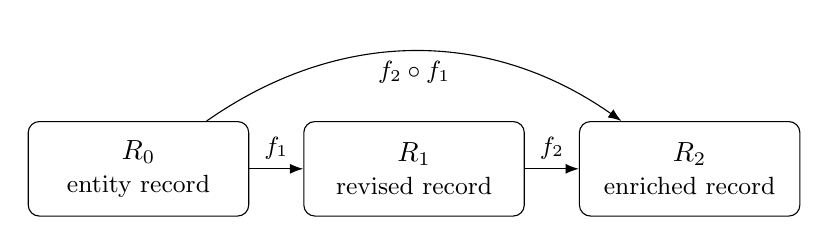
\begin{tikzpicture}[
      node distance=3.5cm,
      state/.style={rectangle,rounded corners,draw,minimum width=2.8cm,minimum height=1.2cm,align=center},
      >=Latex
    ]
    \node[state] (R0) {$R_0$\\{\small entity record}};
    \node[state,right of=R0] (R1) {$R_1$\\{\small revised record}};
    \node[state,right of=R1] (R2) {$R_2$\\{\small enriched record}};

    \draw[->] (R0) -- node[above]{\small $f_1$} (R1);
    \draw[->] (R1) -- node[above]{\small $f_2$} (R2);
    \draw[->, bend left=35]
    (R0) to node[below]{\small $f_2 \circ f_1$} (R2);
  \end{tikzpicture}

  \caption{Morphisms in $\mathbf{CEP}$ as provenance-preserving transformations.
    Each arrow corresponds to a valid record evolution that preserves schema
    validity, revision monotonicity, and canonical identity.}
  \label{fig:cep-morphisms}
\end{figure}

% ------------------------------------------------------------
\subsection*{D.2 Naturality of Attestations}
% ------------------------------------------------------------

Figure~\ref{fig:naturality-attestations} visualizes attestations as a
natural transformation between two envelope functors
$\mathcal{E}, \mathcal{E}' : \mathbf{P} \to \mathbf{E}$.

\begin{figure}[ht]
  \centering
  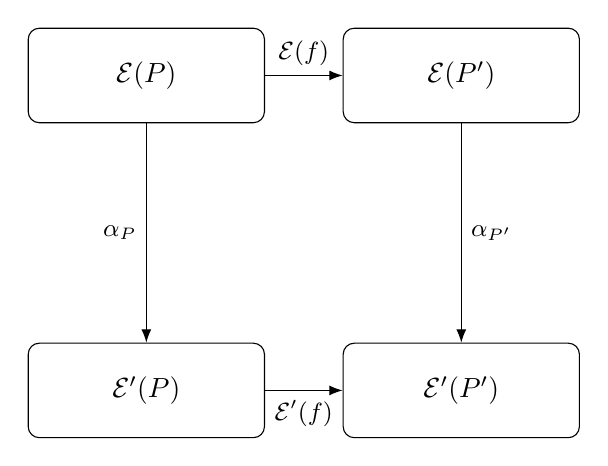
\begin{tikzpicture}[
      node distance=4.0cm,
      obj/.style={rectangle,rounded corners,draw,minimum width=3.0cm,minimum height=1.2cm,align=center},
      >=Latex
    ]
    \node[obj] (EP) {$\mathcal{E}(P)$};
    \node[obj,right of=EP] (EPP) {$\mathcal{E}(P')$};
    \node[obj,below of=EP] (E2P) {$\mathcal{E}'(P)$};
    \node[obj,below of=EPP] (E2PP) {$\mathcal{E}'(P')$};

    \draw[->] (EP) -- node[above]{\small $\mathcal{E}(f)$} (EPP);
    \draw[->] (E2P) -- node[below]{\small $\mathcal{E}'(f)$} (E2PP);
    \draw[->] (EP) -- node[left]{\small $\alpha_P$} (E2P);
    \draw[->] (EPP) -- node[right]{\small $\alpha_{P'}$} (E2PP);
  \end{tikzpicture}
  \caption{Naturality square for attestations.
    The equality
    $\alpha_{P'} \circ \mathcal{E}(f) = \mathcal{E}'(f) \circ \alpha_P$
    expresses that attestation commutes with valid transformations of payloads.}
  \label{fig:naturality-attestations}
\end{figure}

% ------------------------------------------------------------
\subsection*{D.3 Canonicalization Pipeline}
% ------------------------------------------------------------

Figure~\ref{fig:canonicalization-pipeline-appendix} summarizes the canonicalization
pipeline: normalization, assembly, and hashing.

\begin{figure}[ht]
  \centering
  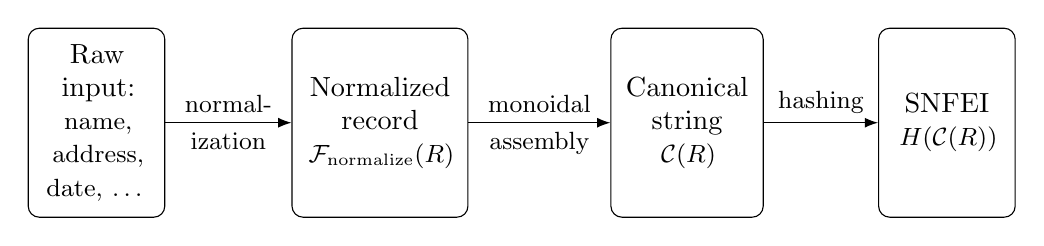
\begin{tikzpicture}[
      stage/.style={
          rectangle,
          rounded corners,
          draw,
          minimum width=1.5cm,
          minimum height=2.4cm,
          align=center
        },
      >=Latex
    ]
    % Explicit positions
    \node[stage, text width=1.5cm] at (0,0)   (raw)   {Raw input:\\{\small name, address, date, \dots}};
    \node[stage, text width=2cm] at (3.6,0) (norm)  {Normalized record\\{\small $\mathcal{F}_{\text{normalize}}(R)$}};
    \node[stage, text width=1.7cm] at (7.5,0)   (canon) {Canonical string\\{\small $\mathcal{C}(R)$}};
    \node[stage, text width=1.5cm] at (10.8,0) (hash) {SNFEI\\{\small $H(\mathcal{C}(R))$}};

    % Arrows from right edge to left edge
    \draw[->] (raw.east)   --
    node[above]{\small normal-}
    node[below]{\small ization}
    (norm.west);
    \draw[->] (norm.east) --
    node[above]{\small monoidal}
    node[below]{\small assembly}
    (canon.west);
    \draw[->] (canon.east) -- node[above]{\small hashing}  (hash.west);
  \end{tikzpicture}
  \caption{The canonicalization pipeline as a composition of a
    normalization functor, a strict monoidal assembly functor, and a
    hashing endofunctor that collapses canonical strings to identifiers.}
  \label{fig:canonicalization-pipeline-appendix}
\end{figure}


% ------------------------------------------------------------
\subsection*{D.4 Jurisdictional Adapters as Oplax Functors}
% ------------------------------------------------------------

Figure~\ref{fig:oplax-adapter-appendix} illustrates the weakened coherence
condition for an oplax functor
$\mathcal{A} : \mathbf{J_{local}} \to \mathbf{J_{global}}$.

\begin{figure}[ht]
  \centering
  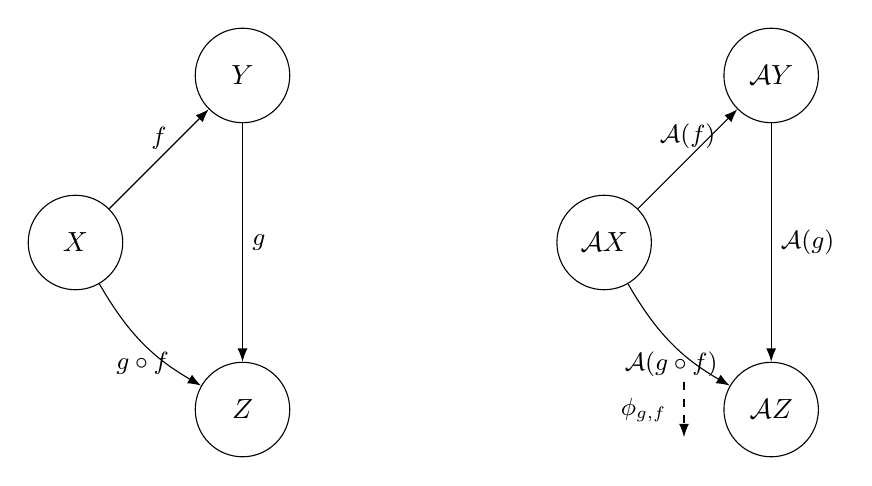
\begin{tikzpicture}[
      node distance=3.0cm,
      obj/.style={circle,draw,minimum size=1.2cm,align=center},
      >=Latex
    ]
    % Local side
    \node[obj] (X) {$X$};
    \node[obj,above right of=X] (Y) {$Y$};
    \node[obj,below right of=X] (Z) {$Z$};

    \draw[->] (X) -- node[above]{\small $f$} (Y);
    \draw[->] (Y) -- node[right]{\small $g$} (Z);
    \draw[->,bend right=15] (X) to node[below]{\small $g \circ f$} (Z);

    % Global side
    \node[obj,right=5.5cm of X] (AX) {$\mathcal{A}X$};
    \node[obj,above right of=AX] (AY) {$\mathcal{A}Y$};
    \node[obj,below right of=AX] (AZ) {$\mathcal{A}Z$};

    \draw[->] (AX) -- node[above]{\small $\mathcal{A}(f)$} (AY);
    \draw[->] (AY) -- node[right]{\small $\mathcal{A}(g)$} (AZ);
    \draw[->,bend right=15] (AX) to node[below]{\small $\mathcal{A}(g \circ f)$} (AZ);

    % Coherence 2-cell: vertical dashed arrow left of AZ
    \draw[->, dashed]
    ($(AZ.west) + (-0.5,0.35)$) -- ($(AZ.west) + (-0.5,-0.35)$)
    node[midway,left,xshift=-0.1cm]{\small $\phi_{g,f}$};

  \end{tikzpicture}
  \caption{Oplax coherence for a jurisdictional adapter
    $\mathcal{A} : \mathbf{J_{local}} \to \mathbf{J_{global}}$.
    The dashed 2-cell $\phi_{g,f}$ witnesses that
    $\mathcal{A}(g \circ f)$ and $\mathcal{A}(g) \circ \mathcal{A}(f)$
    need not coincide strictly, reflecting possible lossy or partial mappings.}
  \label{fig:oplax-adapter-appendix}
\end{figure}

% ------------------------------------------------------------
\subsection*{D.5 Context Tags as a Fibration}
% ------------------------------------------------------------
% Intent: fibers over a base with some functor between them
% Two base objects R and R'
% A base arrow f : R → R'
% Vertical fibers of tags above each
% Solid arrows down to the base (projection)
% Dashed arrows between the fibers (reindexing)
% For a (Grothendieck) fibration
% Given a base arrow  f : R → R'
% standard reindexing is contravariant and we pull back tags along f

Figure~\ref{fig:fibration-ctags} shows the projection
$\pi : \mathbf{CT} \to \mathbf{CEP}$ and the fibers of context tags
above a base record.

\begin{figure}[ht]
  \centering
  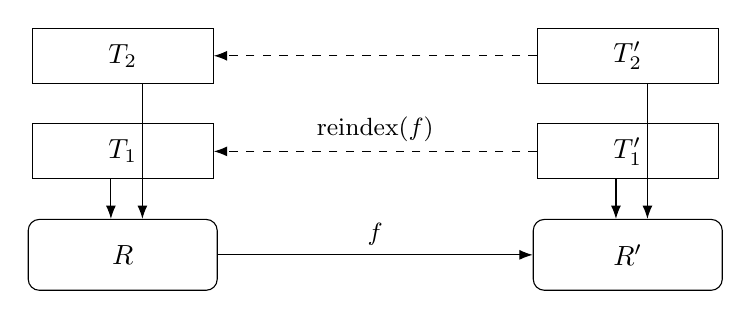
\begin{tikzpicture}[
      node distance=2.4cm,
      base/.style={rectangle,rounded corners,draw,minimum width=2.4cm,minimum height=0.9cm,align=center},
      tag/.style={rectangle,draw,minimum width=2.3cm,minimum height=0.7cm,align=center},
      >=Latex
    ]
    % Base objects
    \node[base] (R) {$R$};
    \node[base,right=4cm of R] (Rp) {$R'$};

    \draw[->] (R) -- node[above]{\small $f$} (Rp);

    % Fiber over R
    \node[tag,above=0.5cm of R] (T1) {$T_1$};
    \node[tag,above=0.5cm of T1] (T2) {$T_2$};

    % Fiber over R'
    \node[tag,above=0.5cm of Rp] (T1p) {$T'_1$};
    \node[tag,above=0.5cm of T1p] (T2p) {$T'_2$};

    % Projections over R
    \draw[->] ($(T1.south) + (-0.15cm,0)$) -- ($(R.north) + (-0.15cm,0)$);
    \draw[->] ($(T2.south) + (0.25cm,0)$)  -- ($(R.north) + (0.25cm,0)$);

    % Projections over R'
    \draw[->] ($(T1p.south) + (-0.15cm,0)$) -- ($(Rp.north) + (-0.15cm,0)$);
    \draw[->] ($(T2p.south) + (0.25cm,0)$)  -- ($(Rp.north) + (0.25cm,0)$);

    % Reindexing along f, fiber over R' -> fiber over R
    \draw[->,dashed] (T1p) -- node[above]{\small $\mathrm{reindex}(f)$} (T1);
    \draw[->,dashed] (T2p) -- (T2);

  \end{tikzpicture}
  \caption{Context tags as a fibration $\pi : \mathbf{CT} \to \mathbf{CEP}$.
    Each base record $R$ has a fiber of permitted tags above it.
    A morphism $f : R \to R'$ induces a reindexing between fibers,
    while the underlying canonical identity remains anchored in the base.}
  \label{fig:fibration-ctags}
\end{figure}
   % Diagrammatic intuition (commutative diagrams)
% !TeX root = 00_cep_semantics.tex
\clearpage
\section*{Appendix E. Glossary for Non-Category Theory Readers}
\addcontentsline{toc}{section}{Appendix E. Glossary for Non-Category Theory Readers}

This appendix provides short, non-technical explanations of the categorical
concepts used in the paper.
The intention is to make the mathematical structure
of CEP more accessible to readers from computer science, data engineering,
public administration, and civic-technology communities.

% ------------------------------------------------------------
\subsection*{E.1 Categories}
A \emph{category} is a mathematical setting that describes:
\begin{itemize}
  \item some \textbf{objects} (things), and
  \item some \textbf{morphisms} (arrows) between them.
\end{itemize}

A category is like a directed graph with rules:
every arrow (morphism) has a source and target,
arrows can be composed,
and each object has an identity arrow that starts from the object, points back to the object, and does nothing.

The latin root \emph{morph} means "form" or "shape",
so a morphism is a way of changing the form of one object into another.

In CEP:
\begin{itemize}
  \item objects = record states,
  \item morphisms = valid record transformations (updates, amendments, joins).
\end{itemize}

Defining CEP as a category formalizes the idea of "things and the allowed changes between them".

% ------------------------------------------------------------
\subsection*{E.2 Functors}
A \emph{functor} is a mapping between categories that preserves structure.
It sends:
\begin{itemize}
  \item each object to another object, and
  \item each morphism to another morphism,
\end{itemize}
in a way that respects composition and identity.

In CEP, a functor often represents a pipeline stage, such as:
\begin{itemize}
  \item wrapping a payload in an envelope,
  \item normalizing noisy text into canonical components,
  \item assembling canonical strings.
\end{itemize}

Functors ensure that if a record evolves legally, its transformed
version evolves legally too.

\emph{Function} and \emph{functor} have the same root and similarities,
but different meanings:
functions map elements within sets,
while functors map objects and morphisms between categories.

% ------------------------------------------------------------
\subsection*{E.3 Natural Transformations}
A \emph{natural transformation} is a structured way of comparing two functors.
If functors are "processing stages", a natural transformation is a
systematic way to convert the output of one stage into the output of another.

In CEP, attestations are modeled as natural transformations:
\begin{itemize}
  \item the envelope functor produces a plain metadata wrapper,
  \item the attested-envelope functor produces a cryptographically validated wrapper.
\end{itemize}

Naturality expresses the idea:
\begin{quote}
  "Whether you process then attest, or attest then process,
  you end up with consistent provenance."
\end{quote}

% ------------------------------------------------------------
\subsection*{E.4 Monoidal Categories}
A \emph{monoidal category} is a category equipped with a notion of
"combining things".

Examples:
\begin{itemize}
  \item strings combine by concatenation,
  \item datasets combine by joining,
  \item workflows combine by sequencing.
\end{itemize}

Canonicalization is the process of converting data into a standard format,
most commonly by selecting a single, preferred output
to represent a piece of content that could have multiple versions.

Canonicalization in CEP is \emph{monoidal} because it combines
individual normalized components into a single canonical string
in a strictly deterministic order.

% ------------------------------------------------------------
\subsection*{E.5 Strict Monoidal Functors}
A \emph{strict monoidal functor} is a functor that preserves the
combination structure \emph{exactly}.

In CEP:
\begin{itemize}
  \item the order of pieces (name, address, date, jurisdiction)
        must always be preserved,
  \item no additional symbols or whitespace are introduced,
  \item the final output is the canonical string fed to the SHA-256 cryptographic hash function.
\end{itemize}

This strictness is what guarantees the stability of the SNFEI identifier.

% ------------------------------------------------------------
\subsection*{E.6 Oplax Functors}
An \emph{oplax functor} preserves structure in a weakened, direction-sensitive way.
The \emph{op} prefix indicates \emph{opposite} directionality and \emph{lax} indicates looseness.
An oplax functor therefore "loosens" structure in a specific direction and
allows "preservation up to a coherence map" rather than strict equality.
A coherence map is a controlled way of relating two structures that are not strictly equal.

It allows:
\begin{itemize}
  \item missing fields,
  \item lossy interpretations,
  \item mappings that preserve meaning but not full structure.
\end{itemize}

Jurisdictional adapters in CEP behave oplaxly because:
\begin{itemize}
  \item local data models may omit fields,
  \item global vocabularies may have stricter typing,
  \item some equivalences hold only "up to" a coherence rule.
\end{itemize}

Oplax behavior models "local autonomy with global convergence".
It means that local jurisdictions can adapt data flexibly
while still ensuring that the global system remains coherent and consistent.

% ------------------------------------------------------------
\subsection*{E.7 Pullbacks (Consistent Joins)}
A \emph{pullback} is the categorical notion of a \emph{consistent join}.

If two data sources both refer to the \emph{same entity or event},
the pullback constructs the most precise version of their agreement.

This formalizes CEP's guarantee that:
\begin{quote}
  Records may be joined only when they assert compatible facts.
\end{quote}

A pullback enables us to formally define the data fusion operation that
combines records from different schemas while preserving:
\begin{itemize}
  \item canonical identity,
  \item vocabulary-governed semantics,
  \item provenance constraints.
\end{itemize}

\emph{Data fusion} refers to the process of integrating multiple data sources
to produce more consistent, accurate, and useful information than that
provided by any individual source.

% ------------------------------------------------------------
\subsection*{E.8 Fibered Categories}
A \emph{fibered category} describes a setting where each object has a
family of additional structures "above it".

CEP is a fibered category.
In CEP:
\begin{itemize}
  \item the base category is $\mathbf{CEP}$,
  \item the fibers contain context tags (CTags).
\end{itemize}

This cleanly separates:
\begin{itemize}
  \item \textbf{identity} (in the base category), and
  \item \textbf{interpretation or annotation} (in the fiber).
\end{itemize}

CTags provide information about a record, without affecting the canonical SNFEI identifier.

% ------------------------------------------------------------
\subsection*{E.9 Universal Properties}
A \emph{universal property} describes an object that is "best" or "most canonical" for a specific purpose.

SNFEI behaves like a universal property construction because:

\begin{itemize}
  \item it is determined by a canonical string,
  \item it is invariant under allowed morphisms,
  \item any other identifier consistent with CEP's invariants must factor uniquely through this construction.
\end{itemize}

This is the mathematical justification enabling us to treat SNFEI
as a stable, verifiable, compositional global identifier.

  % ------------------------------------------------------------
  {\small
    \subsection*{E.10 Summary Table}
    \begin{center}
      \begin{tabular}{p{0.23\linewidth} p{0.35\linewidth} p{0.32\linewidth}}
        \toprule
        \textbf{Concept}        & \textbf{Intuition}       & \textbf{CEP Role}         \\
        \midrule
        Category                & Things, allowed changes  & Record states and updates \\
        Functor                 & Structure-preserving map & Normalization, envelopes  \\
        Natural transformation  & Coherent comparison      & Attestations              \\
        Monoidal category       & Combine things           & Canonical assembly        \\
        Strict monoidal functor & Combine exactly          & SNFEI stability           \\
        Oplax functor           & Weak structure map       & Jurisdiction adapters     \\
        Pullback                & Consistent join          & Merging record fragments  \\
        Fibered category        & Object annotations       & CTags above records       \\
        Universal property      & Optimal construction     & Identifier uniqueness     \\
        \bottomrule
      \end{tabular}
    \end{center}
  }

% ------------------------------------------------------------
\subsection*{E.11 Closing Note}
These notions are not introduced for abstraction's sake;
they express precisely and formally the structural guarantees
CEP requires to support interoperability, trust, and cross-jurisdiction governance.

These mathematical definitions allow the protocol to be:
\begin{itemize}
  \item modular in its design,
  \item formally verifiable in its behavior,
  \item capable of operating consistently even when sources use different schemas, vocabularies, or jurisdictional rules,
  \item and extensible to future domains.
\end{itemize}

By grounding CEP in category theory,
we provide a rigorous foundation for its design principles and operational claims.
   % Glossary of categorical terms for non-specialists

\bibliographystyle{plainnat}
\bibliography{bib_shared}
\end{document}
